\documentclass[letterpaper, 12pt]{amsart}

\usepackage{amssymb}
\usepackage{amsthm}
\usepackage[letterpaper, margin=1.25in]{geometry}
\usepackage{setspace}
\usepackage{verbatim}
\usepackage{tikz}

\onehalfspacing

\title{Path Coloring Algorithms on Plane Graphs}
\author{Aven Bross}

\theoremstyle{definition}
\newtheorem{definition}{Definition}[section]

\theoremstyle{definition}
\newtheorem{example}{Example}[section]

\theoremstyle{thm}
\newtheorem{theorem}{Theorem}[section]

\theoremstyle{definition}
\newtheorem{algorithm}{Algorithm}[section]



\tikzset{%
    every node/.style={circle, fill, draw, minimum size=1mm, scale=.5,
    	font=\LARGE}
}

\begin{document}

\maketitle

\section{Plane Graphs}

A \textit{(simple) graph} $G=(V,E)$ consists of a finite set $V$ of
\textit{vertices} and a set $E$ of two element subsets of $V$ known as
\textit{edges}. We will often refer to the graph as $G$ and the vertex and
edge sets as $V(G)$ and $E(G)$ respectively. As shortand we will denote an edge
$\{u,v\}\in E(G)$ simply as $uv$. Two vertices $u,v\in V(G)$ are
\textit{adjacent} if $uv\in E(G)$. Vertices $u$ and $v$ are known as the
\textit{endpoints} of $uv$. The edge $uv$ is said to be incident to the vertices
$u$ and $v$. The vertices in $G$ adjacent to a vertex $v$ are known as
the \textit{neighbors} of $v$. The \textit{degree} of $v$ is its number of
neighbors, denoted $\text{deg}(v)$.

A graph $H$ is a \textit{subgraph} of $G$ if $V(H)\subseteq V(G)$ and
$E(H)\subseteq E(G)$. If $S\subseteq V(G)$ the \textit{induced subgraph} of
$S$ on $G$ is the subgraph $H$ defined by $V(H)=S$ and
$E(H)=\{uv\in E(G) \ | \ u,v\in S\}$. We say a subgraph $H$ of a graph $G$ is
\textit{induced} if it is the induced subgraph of its vertex set on $G$. If
$v\in V(G)$ we will use $G-v$ to denote the subgraph obtained by removing $v$
and its incident edges from $G$. Similarly, if $H$ is a subgraph of a graph $G$,
we define $G-H$ to be the subgraph obtained by removing from $G$ all vertices in
$H$ and all edges incident to a vertex in $H$.

A length $n$ path consists of the vertices $v_1,v_2,\ldots,v_n$ and the edges $v_1v_2,
v_2v_3,\ldots,v_{n-1}v_n$. A length $n$ cycle, or $n$-cycle, consists of a
length $n$ path and the additional edge $v_1v_n$. We will often denote a path
or cycle $G$ by simply listing its vertices in order, i.e. $G=v_1v_2\ldots v_n$.
If a path $P=v_1v_2\ldots v_n$ is a subgraph of a graph $G$, we say $P$ is a
\textit{$v_1v_n$-path} in $G$. A graph $G$ is \textit{connected} if for every
$u,v\in V(G)$, there exists a $uv$-path in $G$. If any $k$ vertices may be
removed from a graph $G$ with $G$ remaining connected, we say $G$ is
\textit{$k$-connected}.

\begin{comment}
\begin{figure}
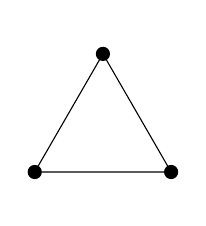
\begin{tikzpicture}
	\node (a) at (0cm,0.75cm) {};
	\node (b) at (0.866cm,-0.75cm) {};
	\node (c) at (-0.866cm,-0.75cm) {};
	\node [draw=none, fill=none] (1) at (0cm,-1cm) {};
	\node [draw=none, fill=none] (2) at (0cm,1cm) {};
	\draw (a) -- (b) -- (c) -- (a);
\end{tikzpicture}
$\qquad$
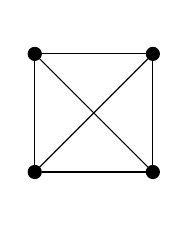
\begin{tikzpicture}
	\node (a) at (0.75cm,0.75cm) {};
	\node (b) at (0.75cm,-0.75cm) {};
	\node (c) at (-0.75cm,-0.75cm) {};
	\node (d) at (-0.75cm,0.75cm) {};
	\node [draw=none, fill=none] (1) at (0cm,-1cm) {};
	\node [draw=none, fill=none] (2) at (0cm,1cm) {};
	\draw (a) -- (b) -- (c) -- (d) -- (a);
	\draw (a) -- (c); \draw (b) -- (d);
\end{tikzpicture}
$\qquad$
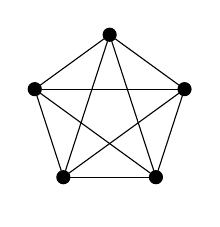
\begin{tikzpicture}
	\node (a) at (90:1cm) {};
	\node (b) at (162:1cm) {};
	\node (c) at (234:1cm) {};
	\node (d) at (306:1cm) {};
	\node (e) at (18:1cm) {};
	\node [draw=none, fill=none] (1) at (0cm,-1cm) {};
	\node [draw=none, fill=none] (2) at (0cm,1cm) {};
	\draw (a) -- (b); \draw (a) -- (c); \draw (a) -- (d); \draw (a) -- (e);
	\draw (b) -- (c); \draw (b) -- (d); \draw (b) -- (e); \draw (c) -- (d);
	\draw (c) -- (e); \draw (d) -- (e);
\end{tikzpicture}
$\qquad$
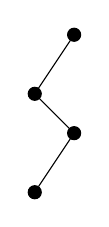
\begin{tikzpicture}
	\node (a) at (0.25cm,1cm) {};
	\node (b) at (-0.25cm,0.25cm) {};
	\node (c) at (0.25cm,-0.25cm) {};
	\node (d) at (-0.25cm,-1cm) {};
	\draw (a) -- (b) -- (c) -- (d);
\end{tikzpicture}
$\qquad$
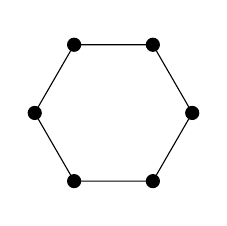
\begin{tikzpicture}
	\node (a) at (180:1cm) {};
	\node (b) at (120:1cm) {};
	\node (c) at (60:1cm) {};
	\node (d) at (0:1cm) {};
	\node (e) at (300:1cm) {};
	\node (f) at (240:1cm) {};
	\node [draw=none, fill=none] (1) at (0cm,-1cm) {};
	\node [draw=none, fill=none] (2) at (0cm,1cm) {};
	\draw (a) -- (b) -- (c) -- (d) -- (e) -- (f) -- (a);
\end{tikzpicture}

\caption{Drawings of $K_3$, $K_4$, $K_5$, a length $4$ path, and a
	$5$-cycle.}
\end{figure}
\end{comment}

A \textit{drawing} of a graph maps each vertex to a point in the
plane and each edge to a curve connecting its endpoints. A \textit{planar
embedding} is a drawing where edge curves intersect only at their
endpoints. We say a graph is \textit{planar} if it admits a planar embedding. A
planar graph together with a planar embedding is a \textit{plane graph}.

Let $G$ be a plane graph. A \textit{face} of $G$ is a maximal region
of the plane not containing any point used in the embedding. The unbounded face
is known as the \textit{outer face}. We will always refer to a face by the
subgraph of vertices and edges that lie on its border. For brevity, we have
not fully formalized curves, regions, or borders. However, the
above definitions and results are fairly standard and may be found in many graph
theory texts, for example \cite{west}.

\begin{theorem}[Euler's Formula]
If $G$ is a connected plane graph with $n$ vertices, $m$ edges, and $f$ faces,
then $n-m+f=2$.
\end{theorem}

A simple corollary of Euler's Formula states that if $n\ge 3$, then $m\le 3n-6$.
A planar graph is said to be \textit{triangulated} if adding any new edge
results in a nonplanar graph. Triangulated plane graphs with $n\ge 3$ vertices
have exactly $3n-6$ edges. A face is said to be a \textit{triangle} if it is a
$3$-cycle. It is easy to see that all faces in a triangulated
plane graph are triangles: if any face has more than three vertices then we may
add an edge curve connecting two face vertices without crossing existing edges.
Conversely if all faces in a plane graph are triangles, then it is triangulated.

\begin{comment}
\begin{figure}
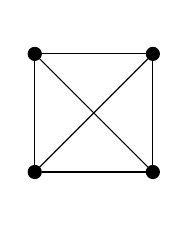
\begin{tikzpicture}
	\node (a) at (0.75cm,0.75cm) {};
	\node (b) at (0.75cm,-0.75cm) {};
	\node (c) at (-0.75cm,-0.75cm) {};
	\node (d) at (-0.75cm,0.75cm) {};
	\node [draw=none, fill=none] (1) at (0cm,-1cm) {};
	\node [draw=none, fill=none] (2) at (0cm,1cm) {};
	\draw (a) -- (b) -- (c) -- (d) -- (a);
	\draw (a) -- (c); \draw (b) -- (d);
\end{tikzpicture}
$\qquad$
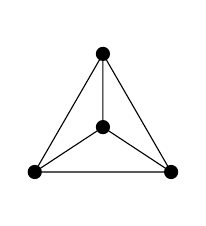
\begin{tikzpicture}
	\node (a) at (0cm,0.75cm) {};
	\node (b) at (0.866cm,-0.75cm) {};
	\node (c) at (-0.866cm,-0.75cm) {};
	\node (d) at (0cm, -0.18cm) {};
	\node [draw=none, fill=none] (1) at (0cm,-1cm) {};
	\node [draw=none, fill=none] (2) at (0cm,1cm) {};
	\draw (a) -- (b) -- (c) -- (d) -- (a);
	\draw (a) -- (c); \draw (b) -- (d);
\end{tikzpicture}

\caption{A nonplanar drawing and a planar embedding of $K_4$.}
\end{figure}
\end{comment}

If a plane graph has triangles for all but one face we shall say it is
\textit{weakly triangulated}. We will always assume the non-triangle face is the
outer face. A $2$-connected weakly triangulated plane graph has a cycle for its
nontriangle face. Suppose $C$ is a cycle in a $2$-connected weakly
triangulated plane graph $G$. Then the subgraph consisting of $C$ and all interior
vertices and edges is denoted $\text{Int}(C)$. If $u,v \in V(C)$ then we denote the $uv$-path in $C$ running
clockwise around the cycle with $C[u,v]$. Finally, if $u,v\in V(C)$ we call any
edge $uv \in E(G)\setminus E(C)$ a \textit{chord} of the cycle $C$.

A \textit{rotation scheme} for a graph $G$ is a cyclic ordering of the incident
edges of each $v\in V(G)$. Planar embeddings naturally induce a rotation
scheme by the counterclockwise order in which edge curves are positioned around
each vertex. In fact, with respect to graph algorithms, the induced rotation
scheme contains all the useful information of an embedding. Therefore, while we
may often visualize plane
graphs with drawings, planar embeddings will always be represented solely by
their induced rotation scheme.

\section{A Brief Review of Coloring Plane Graphs}

A $k$\textit{-coloring} of a graph maps each vertex to one of $k$ possible
colors. Equivalently, a $k$-coloring partitions the vertices of a graph into $k$
disjoint sets called \textit{color classes}. 
A coloring is \textit{proper} if no pair of adjacent vertices recieve the same
color, or equivalently, if the color classes each consist of nonadjacent vertices. It
is clear not all planar graphs admit a proper $3$-coloring since $K_4$ is planar
and requires $4$ colors. Whether all planar graphs admit a proper coloring with
$4$ colors, the Four Color Problem, remained one of the premier open questions
in graph theory until it was verified by Appel and Haken in 1976
\cite{appel1, appel2}.

An $(k,l)$-coloring, or a $k$-coloring with defect $l$, is a
$k$-coloring such that each vertex has at most $l$ same color neighbors.
Generalizations of proper colorings were first introduced by Chartrand et al. in
\cite{chartrand}, while defective, or improper colorings in prticular were introduced
simultaneously by Cowen et al. \cite{cowen}, Jones et al. \cite{jones}, and
Jacobson et al. \cite{jacobson}. It was shown in \cite{cowen} that all
planar graphs admit a $(3,2)$-coloring.

A \textit{path $k$-coloring}, first introduced in \cite{harary}, is a
$k$-coloring such that the induced subgraph of each color class consists of one
or more disjoint paths. Note that path $k$-coloring is equivalent to
$(k,2)$-coloring with the added restriction that path coloring forbids cycles.
Poh \cite{poh} proved that all planar graphs may be path $3$-colored, and this
proof is easily adapted to an algorithm for coloring plane graphs. Here we
provide a naive implementation of Poh's algorithm, running in $\mathcal{O}(n^2)$
time, as well as a more in depth implementation that runs in $\mathcal{O}(n)$.

Let $G$ be a graph and suppose $L$ is a map assigning each vertex $v\in V(G)$ a
list of colors. Then a \textit{$k$-list-coloring} of $G$, first introduced
by Erd{\"o}s et al. in \cite{erdos}, maps each $v\in V(G)$ to a color in $L(v)$.
In \cite{thomassen} Thomassen proved tht all planar graphs may be properly
$5$-list-colored. A planar graph that may not be properly $4$-list colored was
described by Voigt in \cite{voigt}, so Thomassen's result is best possible.

We may equivalently define the defective $(k,l)$-list-colorings and path
$k$-list-colorings. Hull and Eaton \cite{hull} and Skrekovski \cite{skrekovski}
independantly proved that planar graphs are $(3,2)$-list-colorable. Hartman
\cite{hartman}, also independant, described a procedure for path
$3$-list-coloring plane graphs. Interestingly, the proofs of Hartman and
Skrekovski follow the same coloring algorithm, and thus Skrekovski
unknowningly showed the stronger path $3$-list-coloring result. Here we present
an $\mathcal{O}(n)$ implementation of Hartman and Skrekovski's algorithm.

\section{Graph Representations and Time Complexity}

The basic operation for all time complexity discussions shall be a single memory
reference lookup, integer assignment, or comparison between integers. Memory
references are assumed to be integers. We will also treat the allocation of an
array as a basic operation, although the operations for intializing its
elements are counted separately. In accordance with our assumptions above,
removing an element from a linked list or from the back of an array will be
considered to be $\mathcal{O}(1)$.

Let $G$ be a plane graph. Vertices will be represented by integers, that is, we
shall assume $V(G)=\{1,2,\ldots,n\}$. We will always denote
number of vertices in $G$ with $n$ and the number of edges with $m$. Note if
$n\ge 3$ we have $m\le 3n-6$, thus we have $\mathcal{O}(m)= \mathcal{O}(n)$.
Vertex properties will be stored in arrays indexed by vertices. Thus accessing
or comparing vertex properties shall, in general, be constant time. Finally,
colors are assumed to be integers with a coloring of $G$ represented as
a vertex property.

For each $v\in V(G)$ we define a linked list called an
\emph{adjacency list} containing the neighbors of $v$ ordered according to
the rotation scheme of the embedding. The full plane graph $G$ may then
represented by a size $n$ array $\text{Adj}$ of adjacency lists, indexed by vertices.
That is, each $v\in V(G)$ has the adjacency list $\text{Adj}[v]$.

We will often wish for the ability to quickly find a neighbor $u$
in $v$'s adjacency list from $v$'s entry in $u$'s list. To allow this lookup in
$\mathcal{O}(1)$ time for each $v\in V(G)$ we will instead define $\text{Adj}[v]$
to be a linked list of pairs called an \textit{augmented adjacency list}.
At the position of $u$ in $\text{Adj}[v]$ we will also store a reference to
the position of $v$ in $\text{Adj}[u]$. An augmented adjacency list
representation of a graph $G$ may be constructed from a standard adjacency list
representation in $\mathcal{O}(m)$ time via the following algorithm due to 
Glenn Chappell.\\

\noindent\textbf{Implementation 3.1.} (Augmenting Adjacency Lists)

\noindent\textbf{Input:} An adjacency list representation $\text{Adj}$ of a
graph $G$.

\noindent\textbf{Output:} An augmented adacency list representation
$\text{Adj}'$ of $G$.

\noindent\textbf{Descritpion:} We will begin by using $\text{Adj}$ to construct
an augmented adjacency list representation $\text{Adj}'$ of $G$ with the
reference portion of each node uninitialized.
Next we construct an array $\text{Wrk}[v]$ of size $\text{deg}(v)$ for each
$v\in V(G)$.

We fill in $\text{Wrk}$ as follows. For each $v$ from $1$ to $n$ let us walk
through $\text{Adj}'[v]$. At each neighbor $u$ in $\text{Adj}'[v]$ let
$r_{v,u}$ be the reference to $u$'s position in $\text{Adj}'[v]$ and append the
pair $(v,r_{v,u})$ to $\text{Wrk}[u]$.

After this process finishes each $u\in V(G)$ will have an array $\text{Wrk}[u]$
containing the pairs $(v,r_{v,u})$ for each neighbor $v$, sorted in ascending by
the vertices $v$. We will now initialize the references of each node of the
augmented adjacency lists.

We iterate through the vertices in descending order. Let $v$ be the current
vertex. For each 
$uw\in E(G)$ such that $u<w$ and $v<w$ we shall have initialized the reference
for $u$ in $\text{Adj}'[w]$ and the reference for $w$ in $\text{Adj}'[u]$. We
will also have removed the entry $(w,r_{w,u})$ from $\text{Wrk}[u]$. It remains
to handle edges $uv\in E(G)$ with $v>u$.

For each $v$ from $n$ to $1$ we will walk through $\text{Wrk}[v]$. For $i$ from
$1$ to $\text{deg}(v)$ take $(u,r_{u,v})=\text{Wrk}[v][i]$. Note $u<v$ by our
assumptions above. Moreover, $\text{Wrk}[u]$ contains no entries for neighbors
greater than $v$ so $(v,r_{v,u})$ is the last element of $\text{Wrk}[u]$. Thus
we may lookup $r_{v,u}$ to find $u$'s node in $\text{Adj}'[v]$ and initialize the
reference with $r_{u,v}$. We may similarly initialize the reference for $v$'s
node in $\text{Adj}'[u]$. Finally, we remove $(v,r_{v,u})$ from $\text{Wrk}[u]$.

\noindent\textbf{Time Complexity:} For each edge $uv\in E(G)$ we make a constant
number of assignments to $\text{Adj}'$ and $\text{Wrk}$, two reference
lookups, and one entry removal from the back of $\text{Wrk}[u]$.
Therefore the overall complexity of the algorithm is
$\mathcal{O}\left(\sum_{k=1}^m 1\right)=\mathcal{O}(m)$.\\

If $G$ is a planar graph without a given embedding we may still construct an
adjacency list representation of $G$, with neighbors simply listed in arbitrary
order. There exist numerous algorithms to then simultaneously find an embedding
of $G$ and construct an embedding ordered adacency list representation of the
corresponding plane graph in $\mathcal{O}(n)$ time \cite{tarjan, lempel, boyer,
booth}. Moreover, there exist $\mathcal{O}(n)$ algorithms to add edges
to the adjacency list representation in order to connect, $2$-connect, or
triangulate $G$ while maintaining planarity \cite{hagerup,reed,eswaran}. Thus while algorithms will
often assume input graphs are triangulated and plane embedded, arbitrary planar
graphs may be modified in linear time to fit these criteria.

Finally, for each vertex $v$ we will also store a pair of references to nodes in
$\text{Adj}[v]$. Because the rotation scheme is meant to be a cyclic ordering,
this will allow us to indicate start and stop nodes for traversing each adjacency
list. This will track the ``orientation" of each adjacency list around its
respective vertex.

\begin{comment}
If $G$ is a $2$-connected weakly triangulated graph with an outer cycle
$C=v_1v_2\ldots v_k$, vertices listed in clockwise order. We shall set the
the neighbor range of $v_i$ such that the start and indices are the indices of
$v_{i-1}$ and $v_{i+1}$ in $A[v_i]$, respectively. These indices are consider
in a cyclic manner, that is we consider $v_{0}=v_k$, $v_1=v_{k+1}$, and so on.
Many of the algorithms considered will work by removing one vertex at a time,
and considering the remaining graph using the maximal $2$-connected
subgraphs. If $v$ on the outer face, we may remove $v$ from $G$ by contracting
the neighhbor ranges for its neighboring vertices on the outer face exclude $v$.
Interior neighborrs will be If one of the
neighbors of $v$ is a cutvertex once $G$ is removed, we will split into two
\end{comment}


\section{Path 3-Coloring}

\begin{comment}
\begin{proof}
If $|V(G)|\le 3$ there are no vertices to color. Let $|V(G)|>3$ and
suppose the theorem holds for all graphs $H$ with $|V(H)|<|V(G)|$. Let
$P=p_0\ldots p_n$ and $Q=q_0\ldots q_m$ denote the two induced paths from the
$2$-coloring of $C$, ordered such that the edges $p_0q_0$ and $p_nq_m$ are in
$C$. Suppose there exist uncolored vertices, that is $V(G)\setminus V(C)\ne
\emptyset$.

Let $t_0$ be the vertex forming a face with $p_0$ and $q_0$. If
$t_0\in P$, this face is already colored and we consider the graph bounded by
$P-p_0$ and $Q$. Similarly, if $t_0\in Q$ then the inductive hypothesis applies
to the graph bounded by $P$ and $Q-q_0$. Let $t_1$ be the vertex forming a face
with $p_n$ and $q_m$ and proceed in the same manner until $t_1$ is not in either
path.

Suppose there exists an induced path $T$ from $t_0$ to $t_1$. We color
$T$ the remaining color not assigned to $P$ or $Q$ and apply the inductive
hypothesis to the subgraph bounded by $P$ and $T$, and the subgraph bounded by
$T$ and $Q$. With only the path $T$ in common between the two subgraphs, the
combined $3$-coloring forms a path coloring of $G$.

Suppose no such path exists from $t_0$ to $t_1$. Since $G$ is weakly
triangulated there must exist an edge $p_iq_j\in E(G)\setminus E(C)$ with
$p_i\in P$ and $q_j\in Q$. We separately apply the inductive hypothesis to the
subgraph bounded by $p_0\ldots p_i$ and $q_0\ldots q_j$, and the subgraph
bounded by $p_i\ldots p_n$ and $q_j\ldots q_m$. The two subgraphs only share the
vertices $p_i$ and $q_j$, thus the combined $3$-coloring forms a path coloring
of $G$.
\end{proof}
\end{comment}

In this section we detail two implementations of an algorithm for path
$3$-coloring plane graphs. We begin by describing the general algorithm proposed
by Poh \cite{poh}.\\

\noindent\textbf{Algorithm 4.1.} (Poh $3$-Coloring)

\noindent\textbf{Input:} A $2$-connected weakly triangulated plane graph $G$
with outer cycle $C=v_1v_2\ldots v_k$ and a $2$-coloring of $C$ such that the
color classes induce the paths $P=v_1v_2\ldots v_l$ and
$Q=v_{k}v_{k-1}\ldots v_{l+1}$.

\noindent\textbf{Output:} A path $3$-coloring of $G$ such that no vertex in
$C$ recieves a same color neighbor in $G-C$.

\noindent\textbf{Description:} If $G-C$ is empty there are no vertices remaining
to color. Otherwise the algorithm proceeds as follows.

Suppose there is a chord of $C$, that is, an edge $v_iv_j\in E(G)\setminus E(C)$
with $i<j$. Since $P$ and $Q$ are induced paths it must be that $v_i\in P$ and
$v_j\in Q$. Let $C_1$ by the cycle consisting of $C[v_j,v_i]$ and the
edge $v_iv_j$, and $C_2$ the cycle consisting of $C[v_i,v_j]$ and the edge
$v_iv_j$. Observe $C_1$ and $C_2$ are each $2$-colored
such that each color class induces a path. Thus we may apply the algorithm to
path $3$-color $\text{Int}(C_1)$ and $\text{Int}(C_2)$. Since the subgraphs
$\text{Int}(C_1)$ and $\text{Int}(C_2)$ have only the vertices of the chord
$v_iv_j$ in common, the combined coloring forms a path $3$-coloring of $G$.

Suppose no chords of $C$ exist. Let $u$ be the neighbor of $v_k$ immediately
clockwise from $v_1$ and let $w$ be the neighbor of $v_l$ immediately clockwise
from $v_{l+1}$. That is, $u,w\in\text{Int}(C)$ are the unique, but possibly not
distinct, vertices such that
the cycles $uv_1v_k$ and $uv_lv_{l+1}$ are both triangles.

Since $G$ is weakly triangulated, $G-C$ is nonempty,
and $C$ has no chords, $G-C$ is connected. Thus there exists a $uw$-path in
$G-C$. Let $T$ be the shortest such path, and note that therefore $T$ is
an induced path. Color $T$ with the remaining color not used on $P$ or $Q$.

Let $C_1$ be the cycle
consisting of $P$, $T$, and the edges $v_1u$ and $v_lw$. Similarly, let $C_2$ be
the cycle consisting of $T$, $Q$, and the edges $v_ku$ and $v_{l+1}w$. Then we
may apply the algorithm to path $3$-color $\text{Int}(C_1)$ and
$\text{Int}(C_2)$. Since $\text{Int}(C_1)$ and $\text{Int}(C_2)$ have only the
vertices of the path $T$ in common, the combined coloring forms a path
$3$-coloring of $G$.\\

\begin{figure}
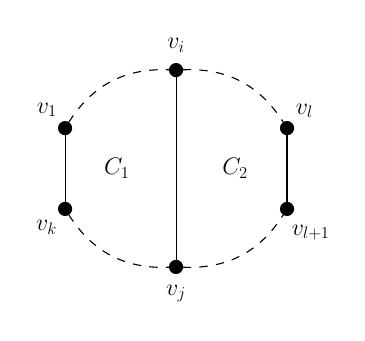
\begin{tikzpicture}
  \node (p0) [label=above left:$v_1$] at (160:1.5cm) {};
  \node (p1) [label=above:$v_i$] at (90:1.25cm) {};
  \node (pn) [label=above right:$v_l$] at (20:1.5cm) {};
  \node (q0) [label=below left:$v_{k}$] at (200:1.5cm) {};
  \node (q1) [label=below:$v_j$] at (270:1.25cm) {};
  \node (qn) [label=below right:$v_{l+1}$] at (340:1.5cm) {};
  \node (null) [draw=none, fill=none] at (270:1.75cm) {};
  
  \node (C1) [draw=none, fill=none] at (180:0.75cm) {$C_1$};
  \node (C2) [draw=none, fill=none] at (0:0.75cm) {$C_2$};
  
  \draw (p0) edge [bend left] (p1) [dashed];
  \draw (p1) edge [bend left] (pn) [dashed];
  \draw (q0) edge [bend right] (q1) [dashed];
  \draw (q1) edge [bend right] (qn) [dashed];
  \draw (p0) edge (q0);
  \draw (pn) edge (qn);
  \draw (p1) edge (q1);
\end{tikzpicture}
$\qquad$
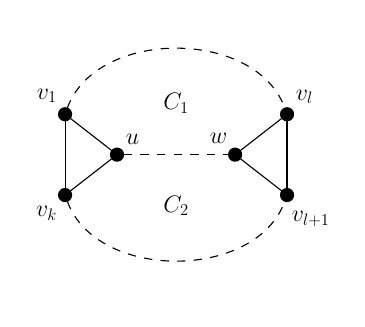
\begin{tikzpicture}
  \node (p0) [label=above left:$v_1$] at (160:1.5cm) {};
  \node (pn) [label=above right:$v_l$] at (20:1.5cm) {};
  \node (q0) [label=below left:$v_{k}$] at (200:1.5cm) {};
  \node (qn) [label=below right:$v_{l+1}$] at (340:1.5cm) {};
  \node (t0) [label=above right:$u$] at (180:0.75cm) {};
  \node (t1) [label=above left:$w$] at (0:0.75cm) {};
  \node (null) [draw=none, fill=none] at (270:1.75cm) {};
  
  \node (C1) [draw=none, fill=none] at (90:0.65cm) {$C_1$};
  \node (C2) [draw=none, fill=none] at (270:0.65cm) {$C_2$};
  
  \draw (p0) edge [bend left=70] (pn) [dashed];
  \draw (q0) edge [bend right=70] (qn) [dashed];
  \draw (p0) edge (q0);
  \draw (pn) edge (qn);
  \draw (p0) edge (t0);
  \draw (q0) edge (t0);
  \draw (pn) edge (t1);
  \draw (qn) edge (t1);
  \draw (t0) edge (t1) [dashed];
\end{tikzpicture}

\caption{The case of a chord (left) and the case no chord exists (right).}
\end{figure}

Given any plane graph $G$ we may add edges until it is triangulated. Observe
that any path coloring of $G$ with the additional edges is also a path coloring
of the original $G$. Therefore by coloring two vertices of the outer
triangle with one color and the remaining outer triangle vertex with another, we
may apply Poh's algorithm to path $3$-color $G$. This observation yields the
following result.

\begin{theorem}[Poh \cite{poh}]
All planar graphs are path $3$-colorable.
\end{theorem}

In order to implement Poh's algorithm there are two main obstacles. Firstly, we
must have a method to efficiently represent induced paths and subgraphs, as we
will be recursively constructing paths and dividing the graph along them.
Secondly, we will need an efficient algorithm to locate chords and $uw$-paths.

In order to efficiently represent induced paths in $G$ we will define a vertex
property $\text{Mrk}[v]$ for each $v\in V$. To represent an
induced path $P=v_1v_2\ldots v_k$ in $G$ we store at the vertices $v_1$ and
$v_k$ as well as an integer $I_P$. We then assign $\text{Mrk}[v_i]=I_P$ for
each $v_i\in V(P)$. Each induced path constructed shall have a unique integer
$I_P$. However, we may subdivide this path, when we split along a chord for
example, by assigning different start and end vertices. So two represented paths
will have the same mark only if they are segments of a larger induced path and
are either disjoint or intersect at a single endpoints.

All paths and cycles discussed as input will be assumed to be subgraphs of a
weakly triangulated plane graph $G$ which we are working to color. We will now
describe our first implementation of Poh's algorithm which uses a breadth first
search to find induced paths and chords.\\

\noindent\textbf{Implementation 4.2.} (Poh -- Breadth First Search)

\noindent\textbf{Assumptions:} Suppose $P=v_1v_2\ldots v_l$ and
$Q=v_kv_{k-1}\ldots v_{l+1}$ are induced
paths such that $C=v_1v_2\ldots v_k$ is a cycle. Finally, assume each
path has been colored with a distinct color.

\noindent\textbf{Input:} The paths $P$ and $Q$.

\noindent\textbf{Output:} We find an extension of the path $2$-coloring of $C$ to
a path $3$-coloring of $\text{Int}(C)$ such that
no vertex in $C$ recieves a same color neighbor in $\text{Int}(C)-C$.

\begin{figure}
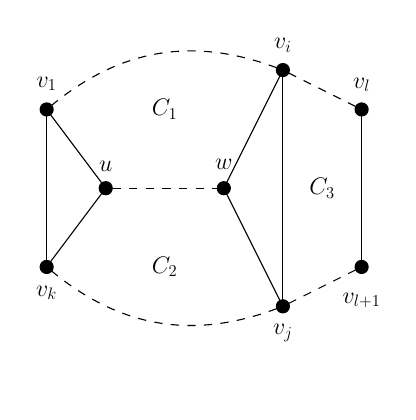
\begin{tikzpicture}
  \node (p0) [label=above:$v_l$] at (2cm, 1cm) {};
  \node (pn) [label=above:$v_1$] at (-2cm, 1cm) {};
  \node (q0) [label=below:$v_{l+1}$] at (2cm, -1cm) {};
  \node (qn) [label=below:$v_k$] at (-2cm, -1cm) {};
  \node (t0) [label=above:$w$] at (0.25cm, 0cm) {};
  \node (t1) [label=above:$u$] at (-1.25cm, 0cm) {};
  \node (pi) [label=above:$v_i$] at (1cm, 1.5cm) {};
  \node (qj) [label=below:$v_j$] at (1cm, -1.5cm) {};
  
  \node (CP) [draw=none, fill=none] at (-0.5cm, 1cm) {$C_1$};
  \node (CQ) [draw=none, fill=none] at (-0.5cm, -1cm) {$C_2$};
  \node (Ci) [draw=none, fill=none] at (1.5cm, 0cm) {$C_3$};
  
  \node (null) [draw=none, fill=none] at (270:2.5cm) {};
  
  \draw (p0) edge (pi) [dashed];
  \draw (pi) edge [bend right] (pn) [dashed];
  \draw (q0) edge (qj) [dashed];
  \draw (qj) edge [bend left] (qn) [dashed];
  \draw (p0) edge (q0);
  \draw (pn) edge (qn);
  \draw (pi) edge (qj);
  \draw (pn) edge (t1);
  \draw (qn) edge (t1);

  \draw (t1) edge (t0) [dashed];
  \draw (pi) edge (t0);
  \draw (qj) edge (t0);
\end{tikzpicture}
$\qquad$
\begin{tikzpicture}
  \node (null) [draw=none,fill=none, scale=2] at (0cm, 0cm) {$\rightarrow$};
  \node (null) [draw=none, fill=none] at (270:2.5cm) {};
\end{tikzpicture}
$\qquad$
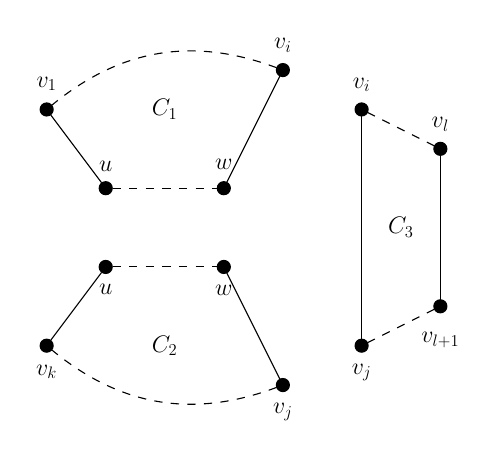
\begin{tikzpicture}
  \node (p0) [label=above:$v_l$] at (3cm, 1cm) {};
  \node (q0) [label=below:$v_{l+1}$] at (3cm, -1cm) {};
  \node (pi) [label=above:$v_i$] at (2cm, 1.5cm) {};
  \node (qj) [label=below:$v_j$] at (2cm, -1.5cm) {};
  
  \node (pi_1) [label=above:$v_i$] at (1cm, 2cm) {};
  \node (pn) [label=above:$v_1$] at (-2cm, 1.5cm) {};
  \node (t0) [label=above:$w$] at (0.25cm, 0.5cm) {};
  \node (t1) [label=above:$u$] at (-1.25cm, 0.5cm) {};
  
  \node (CP) [draw=none, fill=none] at (-0.5cm, 1.5cm) {$C_1$};
  \node (CQ) [draw=none, fill=none] at (-0.5cm, -1.5cm) {$C_2$};
  \node (Ci) [draw=none, fill=none] at (2.5cm, 0cm) {$C_3$};
  
  \node (qj_1) [label=below:$v_j$] at (1cm, -2cm) {};
  \node (qn) [label=below:$v_k$] at (-2cm, -1.5cm) {};
  \node (t0_1) [label=below:$w$] at (0.25cm, -0.5cm) {};
  \node (t1_1) [label=below:$u$] at (-1.25cm, -0.5cm) {};
  \node (null) [draw=none, fill=none] at (270:2.5cm) {};
  \draw (p0) edge (pi) [dashed];
  \draw (pi_1) edge [bend right] (pn) [dashed];
  \draw (q0) edge (qj) [dashed];
  \draw (qj_1) edge [bend left] (qn) [dashed];
  \draw (p0) edge (q0);
  \draw (pi) edge (qj);
  \draw (pn) edge (t1);
  \draw (qn) edge (t1_1);
  \draw (t1) edge (t0) [dashed];
  \draw (t1_1) edge (t0_1) [dashed];
  \draw (pi_1) edge (t0);
  \draw (qj_1) edge (t0_1);
\end{tikzpicture}

\caption{Dividing $G$ along the edge $v_iv_j$ and the $uw$-path.}
\end{figure}

\noindent\textbf{Description:} Locate the position of $v_k$ in $\text{Adj}[v_1]$,
generally this will be given as part of the input. Proceeding one vertex further
in $\text{Adj}[v_1]$ gives us a vertex $u$ such that the cycle $uv_1v_k$ is a triangle. If
$u$ is in $P$, i.e. $u=v_2$, the triangle is colored and we apply the algorithm
to the paths $P-u$ and $Q$. Similarly if $w$ is in $Q$ we apply the algorithm
to $P$ and $Q-u$. In either case, if the two remaining paths each consist of a
single vertex then there are no remaining uncolored vertices and we terminate
the algorithm.

Otherwise, $u$ is an interior vertex. Perform a breadth first search from $u$,
not not including vertices in $C$. Terminate the search when we reach a vertex
$w$ with neighbors $v_i\in P$ and $v_j \in Q$ such that $v_i$ is immediately
past $v_j$ in $\text{Adj}[w]$. Such a vertex must exist
because $\text{Int}(C)$ is weakly triangulated. Backtracking from $w$ along the
breadth first search and
marking vertices produces an induced $uw$-path $T$. We color $T$ with the third
remaining color not used on $P$ or $Q$.

Split $P$ and $Q$ to form the paths $P_1=v_1v_2\ldots v_i$, $P_2=v_ip_{i+1}\ldots v_l$,
$Q_1=v_kv_{k-1}\ldots v_j$, and $Q_2=v_jq_{j-1}\ldots v_{l+1}$. Observe we then
have the cycle $C_1$ consisting of $P_1$, $T$, and the edges $v_1u$ and $v_iw$.
Similarly we have the cycle $C_2$ consisting of $T$, $Q_1$, and the edges $v_ku$
and $v_jw$. We apply the algorithm to $P_1$ and $T$ to color $\text{Int}(C_1)$
and similarly to $T$ and $Q_1$ to color $\text{Int}(C_2)$. If $i=l$ and
$j=l+1$ we are done. Otherwise, we have the cycle $C_3$ consisting of $P_2$,
$Q_2$ and the edges $p_iq_j$ and $p_kq_l$ and we apply the algorithm to $P_2$
and $Q_2$ to color $\text{Int}(C_3)$.

\noindent\textbf{Complexity:} In the first step we rotate through
$\text{Adj}[v_1]$ to find $v_k$ and get an ``orientation" within the graph. This
orientation must be performed at most once for each vertex, for a total of
$\sum_{v=1}^n\text{deg}(v)=2m$ operations.

In the next step we perform a breadth first search from the vertex $u$.
A breadth first search requires at most $n$ lookups. Moreover, the vertex will
$u$ will be colored following the search. Thus we perform at most one breadth
first search from each vertex, requiring at most $n^2$ operations.
Therefore the complexity of the algorithm is at most
$\mathcal{O}(2m + n^2)=\mathcal{O}(n^2)$.

We define the collection of graphs $\{G_k\}_{k\in\mathbb{N}}$, depicted in \ref{poh_example}.
Note $G_k$ has $n=\frac{k^2+k}{2}+3$. The number of operations required will be
$\mathcal{O}\left(\sum_{i=1}^k \frac{k^2+k}{2}\right)=\mathcal{O}(n^{3/2})$.
Thus the complexity of the algorithm is at best $\mathcal{O}(n^{3/2})$. In
particular, the algorithm is not linear.\\

\begin{figure}
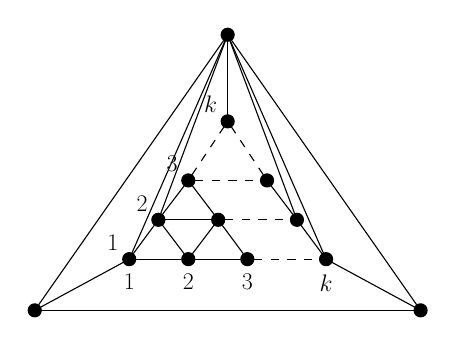
\begin{tikzpicture}
  \node (t1) at (0cm, 3.5cm) {};
  \node (t2) at (2.45cm, 0cm) {};
  \node (t3) at (-2.45cm, 0cm) {};
  
  \node (k1) [label=below:$1$, label=above left:$1$] at (-1.25cm, 0.65cm) {};
  \node (k2) [label=below:$2$]  at (-0.5cm, 0.65cm) {};
  \node (k3) [label=below:$3$]  at (0.25cm, 0.65cm) {};
  \node (kn) [label=below:$k$]  at (1.25cm, 0.65cm) {};
  
  \node (l1) [label=above left:$2$]  at (-0.88cm, 1.15cm) {};
  \node (l2) at (-0.12cm, 1.15cm) {};
  \node (ln) at (0.88cm, 1.15cm) {};
  
  \node (j1) [label=above left:$3$] at (-0.5cm, 1.65cm) {};
  \node (jn) at (0.5cm, 1.65cm) {};
  
  \node (p) [label=above left:$k$]  at (0cm, 2.4cm) {};
  
  \draw (t1) edge (t2); \draw (t3) edge (t2); \draw (t1) edge (t3);
  \draw (k1) edge (k2); \draw (k3) edge (k2);
  \draw (k3) edge (kn) [dashed];
  
  \draw (l1) edge (l2);
  \draw (l2) edge (ln) [dashed];
  
  \draw (j1) edge (jn) [dashed];
  
  \draw (j1) edge (p) [dashed];
  \draw (jn) edge (p) [dashed];
  
  \draw (t1) edge (k1); \draw (t1) edge (kn);
  \draw (t1) edge (l1); \draw (t1) edge (ln);
  \draw (t1) edge (p);
  \draw (t2) edge (kn); \draw (t3) edge (k1);
  
  \draw (k1) edge (l1); \draw (k2) edge (l1);
  \draw (k2) edge (l2); \draw (k3) edge (l2);
  \draw (kn) edge (ln);
  
  \draw (l1) edge (j1); \draw (l2) edge (j1);
  \draw (jn) edge (ln);
  
\end{tikzpicture}

\caption{The collection of graphs $\{G_k\}$ on which Poh performs poorly.}
\label{poh_example}
\end{figure}

Any implementation of Poh's algorithm must find the shortest $uv$-path
within the cycle.
Thus Poh's algorithm does not appear to admit a linear time implementation.

However, that the correctness of Poh's algorithm does not require that $T$
be the shortest $uw$-path, only that $T$ be an induced $uw$-path. We will show that a
linear time implementation exists if we alter Poh's algorithm to instead construct
an induced path by walking along the existing path $P$.\\

\noindent\textbf{Implementation 4.3.} (Poh -- Path Trace)

\noindent\textbf{Assumptions:} Let $P=v_1v_2\ldots v_l$ and
$Q=v_kv_{k-1}\ldots v_{l+1}$ be induced paths such that $C=v_1v_2\ldots v_k$ is
a chordless cycle, and each path has been colored with a distinct color. In
addition, suppose all vertices in $\text{Int}(C)- C$ with a neighbor in $P$
have been marked.

\noindent\textbf{Input:} The vertex $u\in \text{Int}(C)-C$ such that the cycle
$uv_1v_k$ is a triangle.

\noindent\textbf{Output:} We find an induced $uw$-path $T$ colored with a color distinct
from $P$ and $Q$, where $w$ is the vertex in $\text{Int}(C)$ such that the cycle
$wv_lv_{l+1}$ is a triangle.
Let $C_1$ and $C_2$ be defined as usual by splitting along $T$.
We produce a path $3$-coloring of $\text{Int}(C_1)$ such that
no vertex in $C_1$ recieves a same color neighbor in $\text{Int}(C_1)-C_1$,
and similarly for $\text{Int}(C_2)$.

\noindent\textbf{Description:} Intialize $T$ as the path consisting of the
single vertex $u$, coloring $u$ with the designated color. We will recursively
add vertices to $T$ until we reach the vertex $w$.

Suppose we have constructed the induced path $T=t_1t_2\ldots t_d$, with $t_1=u$.
Iterate through $\text{Adj}[t_d]$
beginning from $t_{d-1}$. If we visit a neighbor $v$ that has a neighbor in
$P$ we color $v$, append $T$, and repeat this process with $v$ as the new
end vertex. If we visit $u\in P$ it must be that $t_d=w$ and
the algorithm terminates. Note one of these two cases must occur since $t_d$
has at least one neighbor in $P$.

We first apply \textit{Face Walk} (4.4) to color $\text{Int}(C_2)$. It remains
to color any unocolored vertices in $\text{Int}(C_1)$.

Let $T=t_1t_2\ldots t_d$ be the path constructed above.
For each $p$ from $1$ to $d$ let us iterate through
$\text{Adj}[t_p]$, starting with $t_{p+1}$. In the case $p=d$ we will define
$t_{p+1}=v_l$. Let $j$ be the smallest integer such that $t_{p+1}v_j$ is an edge. Suppose
we visit a neighbor $y\in \text{Int}(C_1)-C_1$ followed by a vertex in $v_i\in P$.
Note by planarity it must be that $i<j$.
We may then apply \textit{Path Trace} (4.3) to color the chordless cycle
$C_y=t_pv_iv_{i+1}\ldots v_jt_{p+1}$, with the vertex $y$ forming the triangle $yt_pv_i$.
Recall all vertices in $\text{Int}(C_y)-C_y$ with neighbors in $P$ have already been
marked.\\

\noindent\textbf{Implementation 4.4.} (Poh -- Face Walk)

\noindent\textbf{Input:} Paths $P=v_1v_2\ldots v_l$ and
$Q=v_kv_{k-1}\ldots v_{l+1}$ forming a cycle $C=v_1v_2\ldots v_k$ satisfying
the requirements of Poh.

\noindent\textbf{Ouptut:} We find an extension of the path coloring of $C$ to
a path $3$-coloring of $\text{Int}(C)$ such that
no vertex in $C$ recieves a same color neighbor in $\text{Int}(C)-C$.

\noindent\textbf{Description:} If $\text{Int}(C)-C$ is empty there is nothing to
color and the algorithm terminates. Otherwise, we proceed as follows.

We will iterate through the vertices of $P$ until we find a chord. All interior
vertices visited will be marked to indicate they have a neighbor in $P$. For
each $i$ from $1$ to $l$ let us walk through
$\text{Adj}[v_i]$ from $v_{i-1}$ to $v_{i+1}$, excluding
$v_{i-1}$ and $v_{i+1}$. For each neighbor $u$ visited,
if $u\not\in C$, then $u\in \text{Int}(C)-C$ and we
mark it. If $u=v_j\in Q$ then $v_iv_j$ is a chord of $C$ and we stop.

We now split $P$ and $Q$ to form the paths
$P_1=v_1v_2\ldots v_i$, $P_2=v_ip_{i+1}\ldots v_l$, $Q_1=v_kv_{k-1}\ldots v_j$,
and $Q_2=v_jv_{j-1}\ldots v_{l+1}$. Let us define $C_1$ and $C_2$ as usual.
We may then apply \textit{Path Trace} (4.3) to color $\text{Int}(C_1)$, and
apply \textit{Face Walk} (4.4) to color $\text{Int}(C_2)$.

\noindent\textbf{Complexity:} Note each vertex will be in precisely one colored
path. During \textit{Path Trace} (4.3) for each vertex $v\in T$ we will iterate through
$\text{Adj}[v]$ at most twice: once to locate the starting neighbor, and once
to simultaneously find the next vertex to add to the path and find uncolored
vertices above $T$. During \textit{Face Walk} (4.5) for each vertex
$v\in P$ we iterate through $\text{Adj}[v]$ at most once. Therefore the complexity of the algorithm is
$\mathcal{O}\left(\sum_{v=1}^n3\cdot\text{deg}(v)\right)=\mathcal{O}(6m)=\mathcal{O}(n)$.



\section{Path 3-List-Coloring}

In this section we describe an implementation of an algorithm for path
$3$-list-coloring plane graphs. The following general algorithm is due to the
independant work of Hartman \cite{hartman} and Skrekovski \cite{skrekovski}.\\

\noindent\textbf{Algorithm 5.1.} (Hartman-Skrekovski -- Path Color)

\noindent\textbf{Input:} Let $G$ be a $2$-connected weakly triangulated plane
graph with outer cycle $C=v_1v_2\ldots v_k$. Let $x=v_1$ and $y\in C-v_1$.
Suppose $L$ is a list assignment for $G$ such that
for each vertex $v\in G$
\[
    \begin{array}{ll}
	    |L(v)|\ge 1 & \text{if } v=x \text{ or } v=y;\\
	    |L(v)|\ge 2 & \text{if } v\in C-x-y;\\
	    |L(v)|\ge 3 & \text{otherwise.}
    \end{array}
\]

\noindent\textbf{Output:} A path $L$-list-coloring of $G$ such that
$x$ and $y$ each recieve at most one same color neighbor.

\noindent\textbf{Description:} Select an arbitrary $c\in L(x)$. We will construct an induced
path $P$ consisting of vertices of $C$, that begins at $x$ and proceeds
clockwise along the outer face a far as possible towards $y$. Initialize $P$ to consist of
the single vertex $x$.

Suppose we have constructed an induced path $P=v_{j_1}v_{j_2}\ldots v_{j_l}$
with $1=j_1<j_2<\ldots<j_l\le k$. Let us select the largest integer $i$ such that
$v_i\in C[v_{j_l},y]$. If no such $i$ exists we have finished constructing $P$.
Otherwise we append $v_i$ to $P$ and repeat.

Let $P=v_{j_1}v_{j_2}\ldots v_{j_l}$ be the path constructed above. For each
$i\in\{1,\ldots,l-1\}$ if $j_i+1<j_{i+1}$ we apply \textit{Remove Path} (5.2)
to the cycle formed by $C[v_{j_i},v_{j_{i+1}}]$ and the edge
$v_{j_i}v_{j_{i+1}}$, with designated vertex $v_{j_i}$.

We finally apply \text{Remove Path} (5.2) to the cycle formed by $P$ and
$C[v_{j_l},v_1]$, with designated vertex $y$.

\noindent\textbf{Algorithm 5.2.} (Hartman-Skrekovski -- Remove Path)

\noindent\textbf{Input:} Let $G$ and $C=v_1v_2\ldots v_k$, $x$, $y$, and $L$ all
be as in (5.1). Suppose $P=v_1v_2\ldots v_l$ is an induced path such that $V(P)
\subseteq V(C[v_1,y])$. Let $P$ be colored with a
color $c$ such that $c\in L(v_i)$ for all $i\in\{1,\ldots,l\}$. Finally, if
$y\not\in P$, suppose for every $v\in C[v_{l+1},y]$, if $v$ has a neighbor in $P$
then $c\not\in L(v)$.

\noindent\textbf{Output:} A path $L$-list-coloring of $G$ such that $v_k$ and
$y$ each recieve at most one same color neighbor, and no vertex in
$G-P$ with a neighbor in $P$ recieves the color $c$.

\noindent\textbf{Description:}
Note $G$ is $2$-connected and weakly triangulated. Thus to disconnect $G$ by
removing vertices from $C$ we would need to remove vertices
$v_i,v_j\in C$ such that $v_iv_j$ is a chord of $C$.
Observe $P$ is an induced path in $C$, so no vertices in $P$ induce a chord of
$C$. So $G-P$ is connected.

Suppose there is a chord of $C$ with an endpoint in $P$. Let us select the
smallest $i\in\{1,\ldots,l\}$ and largest
$j\in\{l+2,\ldots,k-1\}$ such that $v_i\in P$ and $v_iv_j$ is a chord of $C$. Let $C_1$ be the
cycle consisting of $C[v_j,v_i]$ and the edge $v_iv_j$. Similarly, let $C_2$ be
the cycle consisting of $C[v_i,v_j]$ and the edge $v_iv_j$.

We may apply
\textit{Remove Path} (5.2) to $\text{Int}(C_1)$ with $P_{C_1}=v_1v_2\ldots v_i$, $y_{C_1}=v_i$,
and $L_{C_1}=L$. Similalry we may apply (5.2) to $\text{Int}(C_2)$ with
$P_{C_2}=v_iv_{i+1}\ldots v_l$, $y_{C_2}=y$, and $L_{C_2}=L$. Note by our assumptions 

Suppose there are no chords of $C$ with endpoints in $P$.
Then the only neighbors of $P$ in $C-P$ are the vertices $v_k$ and $v_{l+1}$.
Let $L'$ be a list assignment for $G-P$ defined by
\[
	L'(v) = \begin{cases}
				L(v)\setminus\{c\}, \text{if } v \text{ has at least one neighbor in } P;\\
				L(v), \ \text{otherwise}.
			\end{cases}
\]
Let us define the vertex $x'=v_k$. If $y\in P$ we define $y'=v_{l+1}$, otherwise let $y'=y$.
Observe $G-P$ is $2$-connected and $L'$ meets the requirements of \textit{Path Color} (5.1)
with $x'$ and $y'$. We may therefore apply (5.1) to path $L'$-color $G-P$.\\

In order to implement Hartman and Skrekovski's algorithm there are two main
challenges we face. First, we need to be able to remove paths and locate the
remaining blocks for recursive calls. Second, we must be able to track the
location of vertices on the outer face with respect to the designated vertices
$x$, and $y$. For example, when constructing a new path $P$ we need to know if
the vertex we are looking at lies in $C[x,y]$.



\begin{comment}
Let $G$ be a triangulated plane graph with an adjacency list representation.
For each vertex $v$ we will define the vertex property $s$ to mark which
subgraph of $G$ the vertex belongs to. Finally, the vertex property $c$ will
store the color of each vertex. We will describe an algorithm to path $3$ color
following Poh's proof \cite{poh}.

An induced path $v_1v_2\ldots v_n$ in $G$ will be represented by storing the
vertex $v_1$ and an integer $m$. Each $v_i$ will have $s[v_i]=m$. We may walk
through the path one vertex at a time, starting with $v_1$, by looking through
neighbors to find the next marked vertex.

Suppose we have two induced paths $P=p_1p_2\ldots p_k$
and $Q=q_1q_2\ldots q_l$ such that together they form the cycle
$C=p_1p_2\ldots p_kq_lq_{l-1}\ldots q_1$. Moreover, suppose all vertices in $P$
have been colored $c_1$ and all vertices in $Q$ have been colored a color $c_2$,
distinct from $c_1$.

We will color $\text{Int}(C)$ such that no vertex in $C$ recieves a same
color neighbor in $\text{Int}(C)-C$. Locate $u_1$ in $a[v_1]$ by iterating
through the list. Proceeding one vertex further gives us a vertex $w$
such that $p_1q_1w$ is a triangle with no interior vertices. If $w$ is in $P$,
that is $w=p_2$, this triangle has been colored and we may apply the algorithm
to the paths $P-p_1$ and $Q$. Similarly if $w$ is in $Q$ we apply the algorithm
to $P$ and $Q-q_1$. In either case, if the two remaining paths each consist of a
single vertex then there are no remaining uncolored vertices and we terminate
the algorithm.

Otherwise, $w$ is an interior vertex. Perform a breadth first search from $w$,
not not including vertices in $C$, until we reach a vertex $w$ with neighbors
$p_i\in P$ and $q_j \in Q$ such that $p_i$ is immediately past $q_j$ in $a[z]$,
that is, $q_j$ is immediately clockwise from $p_i$. Such a vertex must exist
because $\text{Int}(C)$ is weakly triangulated and the paths $P$ and $Q$ form
the outer cycle. Backtracking from $z$ along the breadth first search and
marking vertices produces an induced $wz$-path denoted $T=t_1t_2\ldots t_r$,
with $t_1=w$ and $t_r=z$. We color this path with the third remaining color
$c_3$.

Let us define the paths $P_1=p_1p_2\ldots p_j$, $P_2=p_jp_{j+1}\ldots p_k$,
$Q_1=q_1q_2\ldots q_j$, and $Q_2=q_jq_{j+1}\ldots q_l$. Observe we then have
the cycle $C_P$ consisting of $P_1$, $T$, and the edges $p_1t_1$ and $p_jt_r$.
Similarly we have the cycle $C_Q$ consisting of $T$, $Q_1$, and the edgess $q_1t_1$ and
$q_jt_r$. We apply the algorithm to $P_1$ and $T$ to color $\text{Int}(C_P)$
and similarly to $T$ and $Q_1$ to color $\text{Int}(C_Q)$. If $i=k$ and
$j=l$ we are done. Otherwise, we have the cycle $C'$ consisting of $P_2$,
$Q_2$ and the edges $p_iq_j$ and $p_kq_l$ and we apply the algorithm to $P_2$
and $Q_2$ to color $\text{Int}(C')$.

\end{comment}


\begin{thebibliography}{21}  % "2" because there are two references
\bibitem{west}
	West, D., \textit{Introduction to Graph Theory},
	2nd ed., Pearson, 2001.
\bibitem{hartman}
	Hartman, C.,
	"Extremal Problems in Graph Theory," Ph.D. Thesis, Department of
	Mathematicsm University of Illinois at Urbana-Champaign, 1997.
\bibitem{skrekovski}
	Skrekovski, R., "List Improper Colourings of Planar Graphs,"
	\textit{Combinatorics, Probability, and Computing}, vol. 8, pp. 293-299,
	1999.
\bibitem{hull}
	Eaton, N., Hull, N., "Defective list colorings of planar graphs,"
	\emph{Bulletin of the Institute for Combinatorics and its Applications},
	1999.
\bibitem{thomassen}
	Thomassen, C., "Every planar graph is 4-choosable,"
	\emph{Journal of Combinatorial Theory Series B}, 1994.
\bibitem{poh}
	Poh, K., "On the linear vertex-arboricity of a planar graph,"
	\emph{Journal of Graph Theory}, vol. 14, pp. 73-75, 1990.
\bibitem{appel1}
	Appel, K., Haken, W., "Every planar map is four colorable. Part I:
	Discharging," \textit{Illinois Journal of Mathematics}, vol. 21, pp. 429-490,
	1977.
\bibitem{appel2}
	Appel, K., Haken, W., "Every planar map is four colorable. Part II:
	Reducibility," \textit{Illinois Journal of Mathematics}, vol. 21, pp.
	491-567, 1977.
\bibitem{chartrand}
	Chartrand, G., Geller, D. P., Hedetniemi, S., "A generalization of the
	chromatic number," \textit{Mathematical Proceedings of the Cambridge
	Philosophical Society}, vol. 64, Cambridge University Press, 1968.
\bibitem{jacobson}
	Andrews, J., Jacobson, M., "On a generalization of chromatic number,"
	\textit{Congressus Numerantium}, vol. 47, pp. 33-48, 1989.
\bibitem{harary}
	Akiyama, J., Exoo, G., Harary, F., "Covering and packing in graphs IV: Linear arboricity,"
	\textit{Networks}, vol. 11, pp. 69-72, 1981.
\bibitem{jones}
	Harary, F., Jones, K., "Conditional colorability II: bipartite variations,"
	\textit{Congressus Numerantium}, vol. 50, pp. 205-218, 1985.
\bibitem{cowen}
	Cowen, L., Cowen, R., Woodall, D., "Defective colorings of graphs in
	surfaces: partitions into subgraphs of bounded valency,"
	\textit{Journal of Graph Theory}, vol. 10, pp. 187-195, 1986.
\bibitem{erdos}
	Erd{\"o}s, P., Rubin, A., Taylor, H., "Choosability in graphs,"
	\textit{Congressus Numerantium}, vol. 26, pp. 125-157, 1979.
\bibitem{voigt}
	Voigt, M., "List colorings of planar graphs,"
	\textit{Discrete Mathematics}, vol. 120, pp. 215-219, 1993.
\bibitem{tarjan}
	Hopcroft, J., Tarjan, E., "Efficient planarity testing," \textit{Journal of
	the ACM}, vol. 21, pp. 549-568, 1974.
\bibitem{lempel}
	Lempel, A., Even, S., Cederbaum, I., "An algorithm for planarity testing of
	graphs," \textit{Theory of graphs: International Symposium}, pp.215-232,
	1967.
\bibitem{booth}
	Booth, K., Lueker, C., "Testing for the consecutive ones property interval
	graphs and graph planarity using PQ-tree algorithms," \textit{Journal of
	Computer and System Sciences}, vol. 13, pp. 335-379, 1976.
\bibitem{boyer}
	Boyer, J., Myrvold, W., "On the cutting edge: simplified $\mathcal{O}(n)$ planarity by
	edge addition," \textit{Journal of Graph Algorithms and Applications}, vol.
	8, pp. 241-273, 2004.
\bibitem{eswaran}
	Eswaran, K., Tarjan, R., "Augmentation problems," \textit{SIAM Journal of
	Computing}, vol. 5, pp. 653-665, 1976.
\bibitem{reed}
	Reed, R., "A new method for drawing a graph given the cyclic order of the
	edges at each vertex," \textit{Congressus Numerantium}, vol. 56, pp.31-44,
	1987.
\bibitem{hagerup}
	Hagerup, T., Uhrig, C., "Triangulating a planar graph," \textit{Library of
	Efficient Datatypes and Algorithms}, software package, Max Planck Institute
	for Informatics, Saarbr{\"u}cken, 1991.
\end{thebibliography}
\end{document}
